\sectionframe{Structure of an OPL project}
\begin{frame}
 \setbeamercovered{transparent}
 \frametitle{Types of OPL files}
 \begin{description}
  \item<1-2>[model files] description of a generic optimization model (extension: \texttt{.mod})
  \item<1-2>[data files] data for instantiation of an OPL model (extension: \texttt{.dat})
  \item<1-1>[settings files] settings for the solver (extension: \texttt{.ops})
 \end{description}
\end{frame}

\begin{frame}
 \frametitle{Structure of an OPL project}
 \begin{figure}
  \centering
  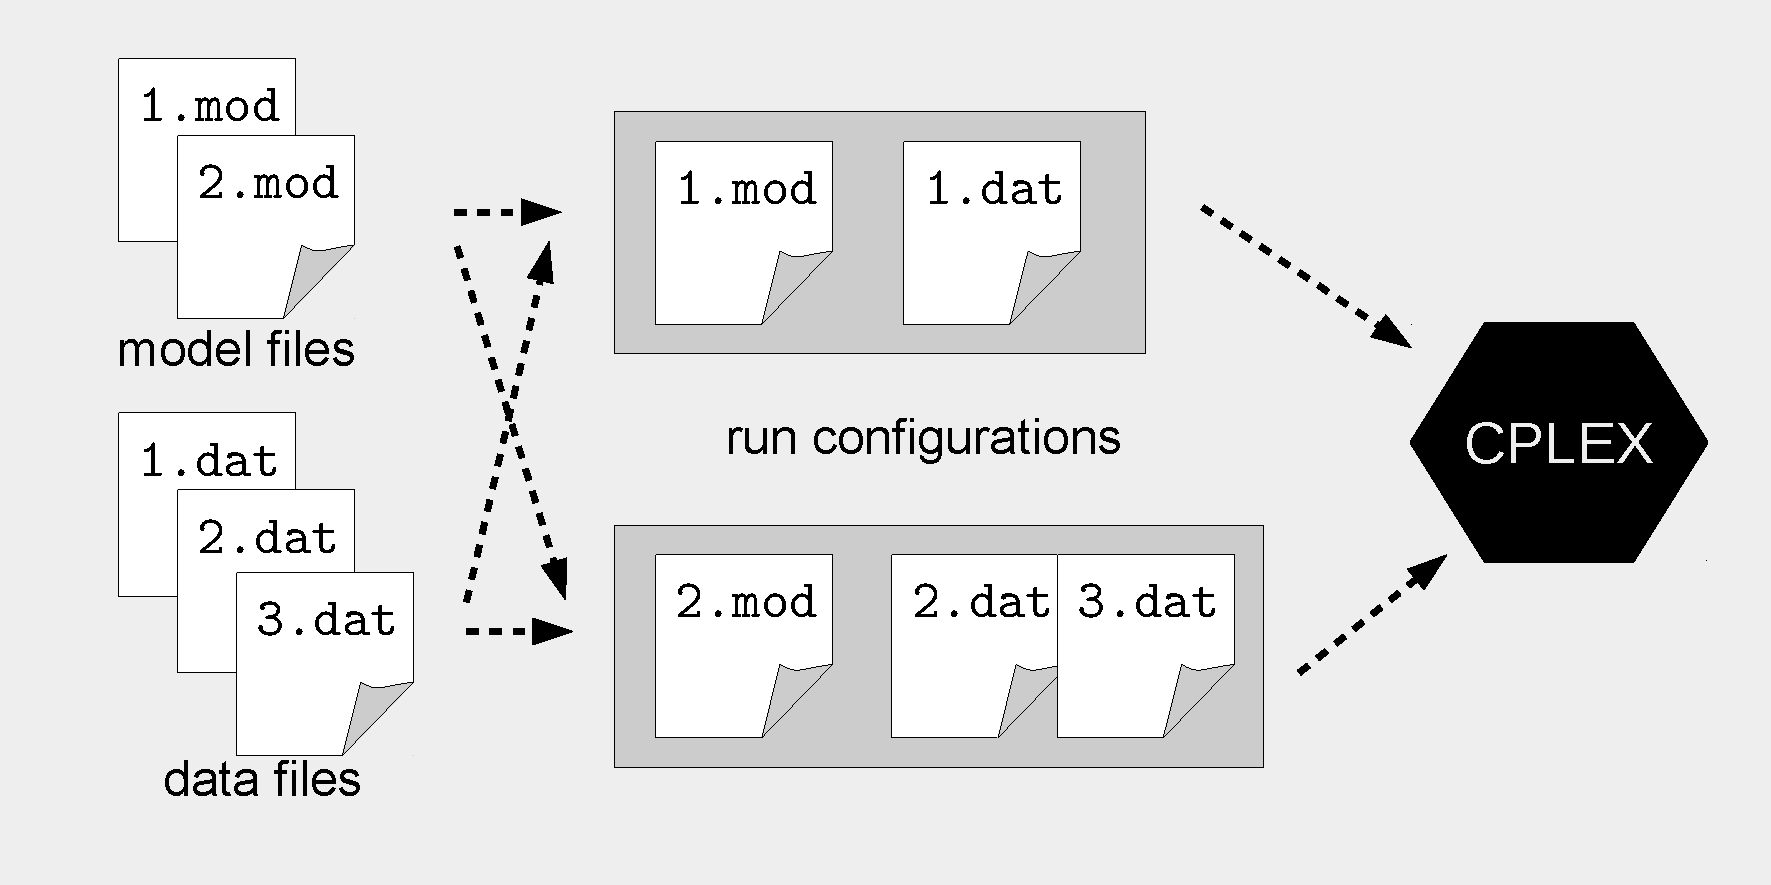
\includegraphics[width=\linewidth]{Bilder/OPL-Aufbau2}
 \end{figure}
\end{frame}
